% \documentclass[11pt]{article}
% \RequirePackage[font=small,labelfont=bf]{caption}
% \RequirePackage{amsmath,amssymb,amsthm}
% \usepackage{graphicx}
% \usepackage{verbatim}
%  \graphicspath{{figs/}} 
%  \usepackage{wrapfig}
% \headheight 0pt \headsep 0pt \oddsidemargin -0.45in \evensidemargin
% -0.45in \textwidth 7.25in \textheight 9.5in \topmargin-0.4in
% \input epsf
% %\pagestyle{empty}
% \begin{document}
% \pagestyle{plain} \footskip 0.5in
% \renewcommand{\thepage}{\arabic{page}}
% \bibliographystyle{amsplain}
% \renewcommand{\P}{\mathbb{P}}
% \newcommand{\R}{\mathbb{R}}
% \newcommand{\E}{\mathbb{E}}


\chapter{An Introduction to Mathematical Concepts}
%\title{Basic Mathematical Concepts for PBG 200A}
%\author{Sebastian J. Schreiber and Graham Coop \\}
%Now, in the first place I deny that the mathematical theory of population genetics is at all impressive, at least to a mathematician. On the contrary, Wright, Fisher, and I all
\begin{quote}
``Now, in the first place I deny that the mathematical theory of
population genetics is at all impressive, [... We] made simplifying assumptions which allowed us to pose problems
soluble by the elementary mathematics at our disposal, and even then
did not always fully solve the simple problems we set ourselves. Our
mathematics may impress zoologists but do not greatly impress
mathematicians.''--\citeauthor{haldane1964defense} 
\end{quote}\marginnote{From Haldane's entertaining response to Mayr's criticism of population genetics. 
\cite{haldane1964defense}}

%\maketitle
Throughout these notes we make use of mathematical concepts, many of
which are based in probability theory and statistics. Here we briefly
review some of these concepts. The wikipedia pages on
statistics and math topics are often excellent introductions, and
worth consulting if you want to know more. This primer was originally written by
Sebastian Schreiber and myself for our Fall quarter of the PBG core
(although I take full credit for any errors subsequently introduced).

%While we might spend some time discussing them in lecture, it probably is a good idea to make sure that you are comfortable with these concepts and if not, talk to one of us about where to read about them online in more detail. 


\section{Calculus}

The \emph{derivative} $f'(a)$ of a function $f(x)$ at $x=a$ represents
the instantaneous rate of change of the function, $\frac{df(x)}{dx}$, at $x=a$ or,
equivalently, the slope of the graph of the function at $x=a$. The
derivative is zero at local maxima and minima of the function,\sidenote{As
  well as saddle points, but we'll not be too concerned about those.} see Figure \ref{Fig:derivative}.
    
\begin{figure}
 \begin{center}
   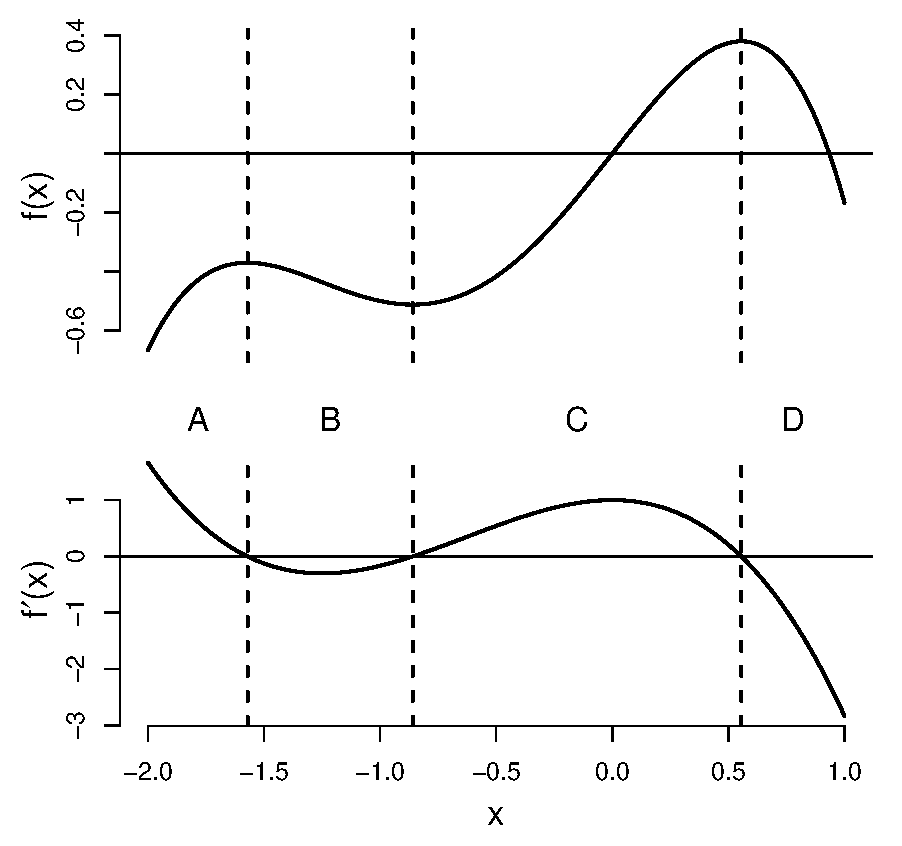
\includegraphics[width=0.7 \textwidth]{math_background/calc_pics/Derivat.pdf}\end{center}
 \caption{{\bf Top)} An example function, $f(x) = x -(\nicefrac{5}{6})x^3  -
   (\nicefrac{1}{3}) x^4$, and {\bf Bottom)} its derivative $f'(a) = 1 - 3(\nicefrac{5}{6}) x^2 -4 (\nicefrac{1}{3}) x^3$
   \gitcode{https://github.com/cooplab/popgen-notes/blob/master/math_background/Calc_background.R}}\label{Fig:derivative}
\end{figure}
To give a physical example, imagine that the derivative of position with respect to
time gives the (instantaneous) speed of a car. Think of the top panel of Figure \ref{Fig:derivative}
as showing a car driving up and down an
alley, the page, with $f(x)$ giving the car's position at time $x$. The bottom panel
shows the car's speed, with the sign (i.e. $\pm$) of the derivative giving the direction of
movement. Moving from left along the $x$ (time) axis, in time period A our car is moving up the alley (page), the speed is
positive (i.e. $f'(a)>0$). In the time period B, the car is reversing down the alley, its speed is negative ($f'(a)<0$ ).  
As we move from A to B the car is beginning to slow down, i.e. the derivative gets small
in magnitude, as it's going to reverse direction at time indicated by
the first dotted line at the point. At the
dotted line between A and B, we are at the moment when the car is changing direction, the car is
stationary, its speed is zero (i.e. $f'(a)=0$ ). 

We'll sometimes want to know about the  \emph{second derivative} of
$f$, denoted by $f''(a)$ or $\frac{d^2f(a)}{d^2x}$. 
The second
derivative measures the rate at which the first derivative is changing
i.e. the concavity/convexity of the function. See Figure \ref{Fig:2nd_derivative}.
 \begin{figure}
 \begin{center}
   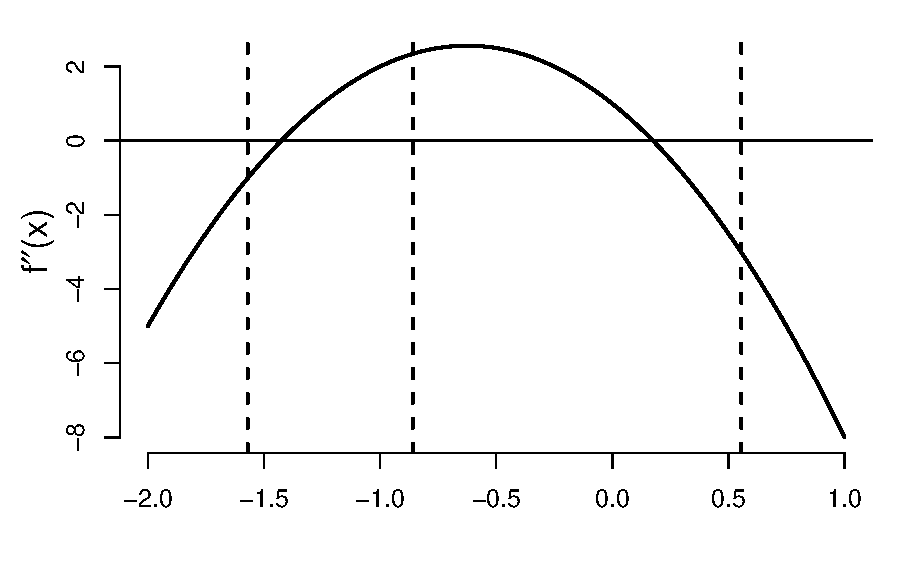
\includegraphics[width=0.7 \textwidth]{math_background/calc_pics/2nd_Derivat.pdf}\end{center}
 \caption{ \gitcode{https://github.com/cooplab/popgen-notes/blob/master/math_background/Calc_background.R}}\label{Fig:2nd_derivative}
 \end{figure}
In our physical example, the second derivative with respect to time is
the (instantaneous) acceleration of the car, as it is the rate of
change in the speed of the car (signed by
whether it's accelerating in a positive or negative direction). One
useful property of the second derivative is that it is positive at
local maxima of the function, and negative for local minima of the function.



%\marginnote{A Taylor series writes a function $$
\subsection{Approximating functions by Taylor Series.}
A wonderful thing about derivatives is that they allow us to approximate
complicated, nonlinear functions by linear functions (this is called a first-order
  Taylor approximation). Namely, a
\emph{first order approximation} of $f(x)$ at $x=a$ is given by 
\begin{equation}
  f(x) \approx f(a)+f'(a)(x-a) \mbox{ for $x$ near $a$}
  \end{equation}
 \begin{marginfigure}
 \begin{center}
   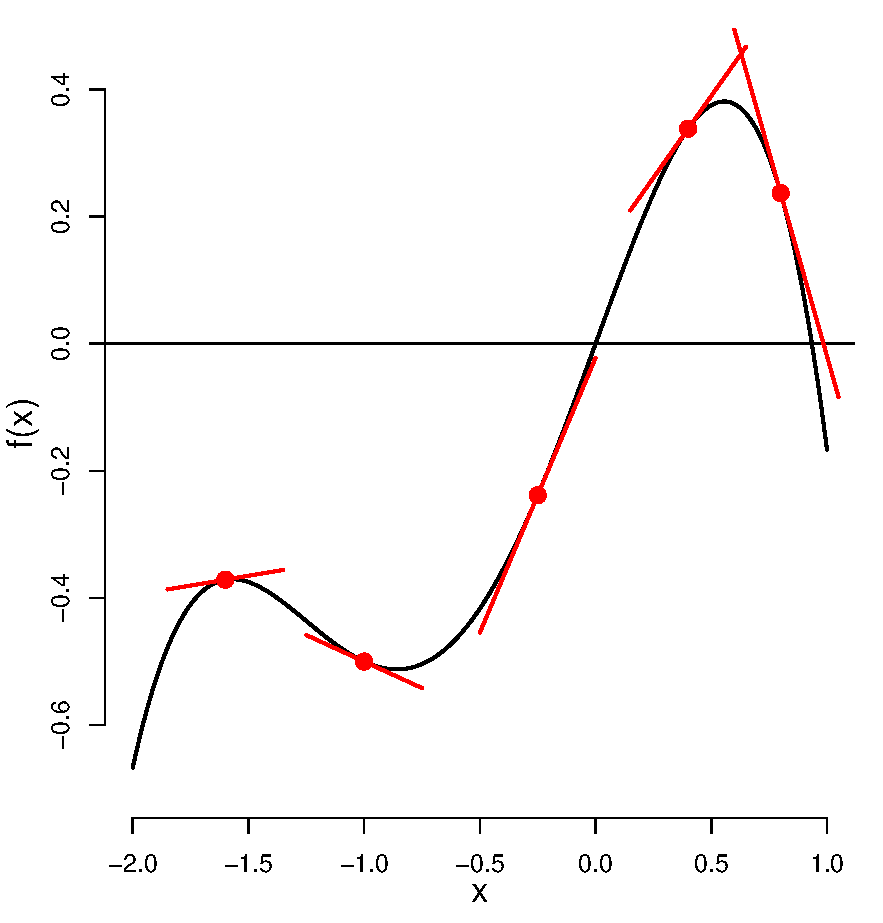
\includegraphics[width=\textwidth]{math_background/calc_pics/Taylor_1.pdf}\end{center}
 \caption{Our function from the top panel of Figure
   \ref{Fig:derivative} approximated by first-order taylor
   approximations (red lines) at a variety of points $a$ (solid
   dots). Note how the approximation breaks down away from the dot, I
   stop plotting the approximation a little away from the dot for easy
   of presentation. \gitcode{https://github.com/cooplab/popgen-notes/blob/master/math_background/Calc_background.R}}\label{FigTaylor_1}
\end{marginfigure}
For example, this approximation yields (\texttt{you can verify this for yourself!}) 
\begin{eqnarray}
\exp(x)&\approx &1+x \mbox{ for $x$ near $0$}\\
(1-x)^k &\approx & 1-k\,x \mbox{ for $x$ near $0$}
\end{eqnarray}

Returning to our car example, this corresponds to trying to guess the
position of the car
extrapolating from its current location and speed. We'll do well when
the car is traveling at a relatively constant speed, i.e. isn't
accelerating or deccelerating too fast. 
 

 \begin{marginfigure}
 \begin{center}
   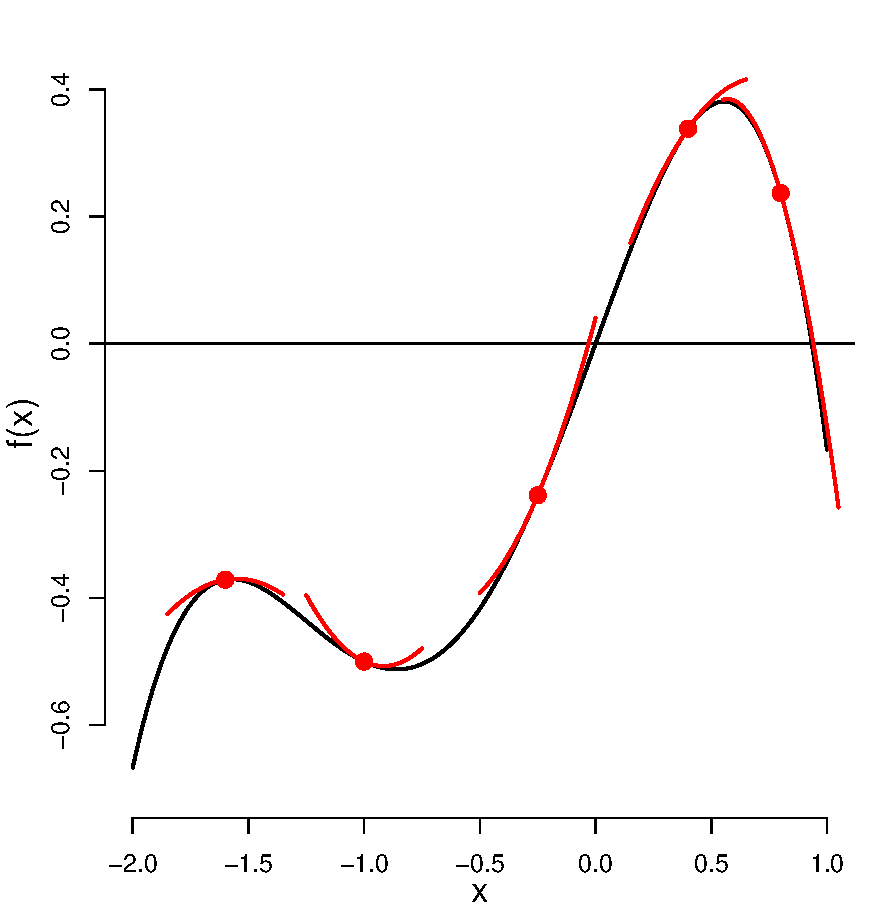
\includegraphics[width=\textwidth]{math_background/calc_pics/Taylor_2.pdf}\end{center}
 \caption{Our function from the top panel of Figure
   \ref{Fig:derivative} approximated by second-order taylor
   approximations (red lines) at a variety of points $a$ (solid
   dots).  \gitcode{https://github.com/cooplab/popgen-notes/blob/master/math_background/Calc_background.R}}\label{FigTaylor_2}
\end{marginfigure}
We'll sometimes want more accuracy and so use a
\emph{second order approximation},
i.e. we will approximate the graph of a function with a parabola instead of a
line (see Figure \ref{FigTaylor_2}). This is often useful when examining the effects of
stochasticity on some process. These second-order Taylor
approximations take the form: 
\begin{equation}
f(x)\approx f(a)+f'(a)(x-a)+f''(a)(x-a)^2/2
\end{equation}
where $f''(a)$ denotes the  \emph{second derivative} of $f$ at
$x=a$. In our car example, this is equivalent to predicting the
location of the car from its speed {\emph and} acceleration. 

This second order approximation is especially useful for the $\log$ function and yields
\begin{equation}
\log(1+x)\approx x-x^2/2 \mbox{ for $x$ near $0$}.
\end{equation}
(\texttt{you can verify this for yourself!})

\subsection{Integrals} Regarding  \emph{integrals} $\int_a^b f(x)\,dx$, just remember that
they represent the \emph{signed area} ``under'' the graph of $y=f(x)$
over the interval $[a,b]$. %It's often helpful to think about an
%integral as 

\section{Probability}

\subsection{Random Variables} A  \emph{random variable} $X$, roughly,
is a variable that takes on values drawn randomly from some
probability distribution.  There are two major types of random
variables, discrete and continuous.  For a discrete random variable, think of it as a person calling out numbers
by drawing them randomly out of a hat with some distribution of
numbered slips of paper. We use $X$ to think about the number that might be drawn (before it is drawn) and x to denote the number that is actually drawn.
%\footnote{Really, to define a random variable, you need a probability space $(\Omega, \Sigma, \P)$ which consists of some event space $\Omega$, a $\sigma$-algebra $\Sigma$ of subsets of $\Omega$ (these correspond to possible events), and $\P$ a probability measure on $\Omega$. A random variable $X$ is a measurable function from $\Omega$  to $\R$. Its probability distribution is determined by $\P(X^{-1}(A))$ for measurable $A\subset \Omega$.}
\emph{Discrete random variables} take on a countable number of values, say $x_1,x_2,\dots$, with some probabilities $p_1,p_2,\dots$. We can denote this assumption as 
\[
\P[X=x_i]=p_i \mbox{ ``the probability that $X$ equals $x_i$ is $p_i$''}
\]

 \emph{Continuous random variables},  which can take on values in a continuum, are
 characterized by their  \emph{probability density function} $p(x)$
 i.e. a function that satisfies $p(x)\ge 0$ for all $x$ and
 $\int_{-\infty}^\infty p(x)\,dx =1$. For example, think about the
 precise time of day a baby
is born in a hospital (not just the hour or the minute, where discrete
random variables would suffice, but the
precise moment). For these variables, 
\[
\P[a\le X\le b] = \int_a^b p(x)\,dx \mbox{ ``the probability that $X$ is interval $[a,b]$ equals the area under the curve $p(x)$ from $a$ to $b$''}
\]
for example, we could ask the probability that a baby was born
somewhere between
midnight and 12.18am. 

\subsection{Basic Rules of Probability}
Imagine a fairground game where you reach into a box and pull out an
egg. There are 100 eggs in the box, 67 of them are empty. Thirty three have a toy in them.
There are eggs with a stuffed dog toy, eggs with a cat toy, eggs with
a lizard toy, eggs with both a dog and cat toy in them. The counts of
each type of egg are shown in Figure \ref{Fig:Venn_toys}.


 \begin{marginfigure}
 \begin{center}
   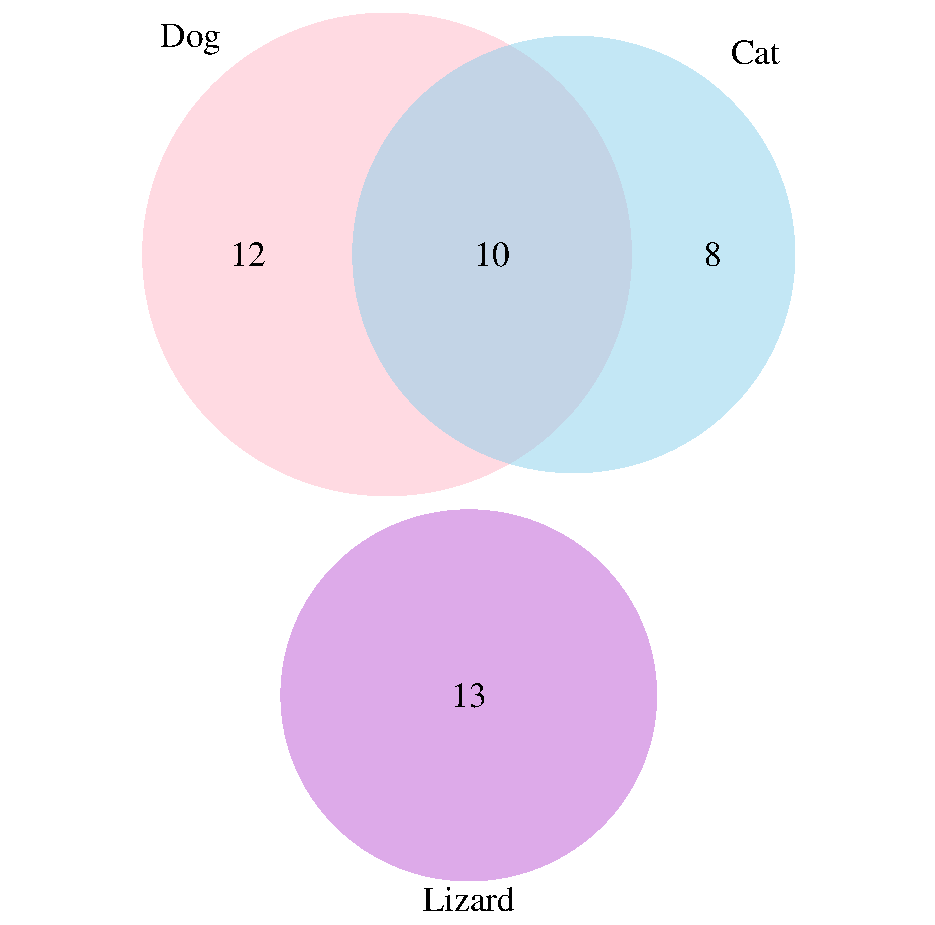
\includegraphics[width=\textwidth]{math_background/dist_pics/Venn_toys.pdf}\end{center}
 \caption{Venn diagram of fairground game toys, there are a hundred
   eggs in total, including 67 eggs with no prize that are not shown. \gitcode{https://github.com/cooplab/popgen-notes/blob/master/math_background/Math-background.R}}\label{Fig:Venn_toys}
 \end{marginfigure}

\begin{question}
You reach into the box and pull out one egg:\\
{\bf i)} For each egg type (dog alone, cat alone, lizard, dog+cat, and no prize),
what is the probability that you get an egg of that type? What do these probabilities sum to?\\
{\bf ii)} What's the probability of getting an egg with a dog? What is
the probability of getting an egg with a dog in it {\it or} an egg without a dog in it. \\
{\bf iii)} What's the probability of getting an egg with a dog in it {\it or} an egg with a lizard. \\
\end{question}
These questions above illustrate the principal that if events A \& B
are mutually exclusive then $\P(\textrm{A or B}) = \P(A) + \P(B)$,
following from these $\P(\textrm{A or not A}) = \P(A) + \P(not A) =
1$. What is the probability of getting an egg with a dog {\it or} a
cat?  Well, for events that are not mutually exclusive we need to
discount the sum of the probabilities by their overlap, giving
\begin{equation}
\P(\textrm{A or B}) = \P(A) +\P(B) - \P(\textrm{A \& B}).
\end{equation}
We call $ \P(\textrm{A \& B}) $ the joint probability of A \& B.
\begin{question}
What is the probability $\P(\textrm{dog or cat})$?
\end{question}


\paragraph{Conditional probability}
We often want to know the probability of an event conditional on some
other particular event, e.g. the probability of getting a cat toy
given that I've pulled out an egg containing a dog (recall that ten of the hundred eggs contain both a dog and a cat toy.). 
We write this as $\P(\textrm{cat} | \textrm{dog})$, where we read $|
\textrm{dog}$ as `given dog' or `conditional on dog'.  The rule of conditional probabilities is that
\begin{equation}
\P(A | B) = \frac{\P(\textrm{A \& B} )}{P(B)}  \label{eqn:cond_prob}
\end{equation}
we can now answer
\begin{question} \label{question:cond}
What is $ \P(\textrm{cat} | \textrm{dog})$?\\
Explain the underlying intuition of your answer? \\
\end{question}
By rearranging eqn \eqref{eqn:cond_prob}, we obtain the rule that
\begin{equation}
\P(\textrm{A \& B}) = \P(A | B) \P(B) .
\end{equation}
Thus we can always obtain the joint probability of A \& B by
multiplying the conditional probability by the probability of the
event we are conditioning on. Equivalently, we could have computed the
joint probability as
\begin{equation}
\P(\textrm{A \& B}) = \P(B | A) \P(A) .
\end{equation}
these two ways of writing the same thing will come in useful in just a
moment.

The total probability of an event can be obtained by summing over
all of the mutually independent ways that A can happen
\begin{equation}
  \P(A)  = \sum_{i=1}^L \P(\textrm{A \& B$_i$}) = \sum_{i=1}^L \P(A | B_i) \P(B_i)  
\end{equation}
where $B_1,~\cdots,~B_L$ give the mutually exclusive events
that can occur alongside our event $B$. This is the \emph{law of total
  probability}. For example, we can write the probability of obtaining
a cat as
\begin{equation}
 \P(\textrm{cat}) = \P(\textrm{cat \& dog}) + \P(\textrm{cat \& not dog}). 
\end{equation}

\paragraph{Independence}
Two events are independent of each other if
\begin{equation}
\P(\textrm{A \& B}) = \P(A) \P(B) \label{eqn:basic_indie}
\end{equation}
this requirement implies independence because the conditional and
unconditional probabilities are equal, $P(A) = P(A | B)$, i.e. I learn
nothing about the event $A$ from the event $B$ having occurred. 
For example, if I draw two eggs with replacement from the box the
probability of getting a lizard then a dog is $\P(\textrm{lizard then} \& \textrm{dog}) =
\P(\textrm{lizard}) \P( textrm{dog})$. 


\paragraph{Bayes Rule}
We often want to reverse of conditional probability statements,
i.e. turn the statement of $P(B | A)$ into the statement of $P(A |
B)$. 
We have two different ways of expressing the joint probability in terms of conditional probabilities. Because they each equal the joint probability, they are equal to each other, meaning
\begin{equation}
\P(B | A) \P(A) =  \P(A | B) \P(B) . \label{eqn:two_joint_probs}
 \end{equation}
Rearranging eqn \eqref{eqn:two_joint_probs} we obtain 
\begin{equation}
\P(B | A) =  \frac{\P(A | B) \P(B) }{\P(A)} \label{eqn:Bayes_Rule}
 \end{equation}
Equation \eqref{eqn:Bayes_Rule} is also called ``Bayes' Rule" or ``Bayes' Theorem," and it  which allows us to reverse the variable we
condition on. 
\begin{question}
Use Bayes' rule to calculate $\P(\textrm{dog} | \textrm{cat})$ from
the conditional probability you calculated in Question
\ref{question:cond}.\\
 \end{question}

\subsection*{Expectation of a Random Variable} The  \emph{expectation
  of a random variable} is the point at which the distribution is
``balanced''. For discrete random variables it is given by 
\begin{equation}
\mu = \E[X]=p_1x_1+p_2x_2+\dots + 
\end{equation}
the expectation of a random variable is the mean of the distribution.
%According to Pascal, it is the excitement a gambler feels when placing
%a bet i.e. each term in the sum equals the probability of winning
%times the amount won.
Our average outcome \footnote{Recalling that we compute average, the sample mean, of a set of numbers $X_1,\cdots,X_L$ as
\begin{equation}
\bar{X} =\frac{1}{L} \sum_{i=1}^L X_i
\end{equation}
where the bar over the $X$ denotes that it is the average value of
$X$.}
over a set of independent
events is an estimate of the mean $\hat{\mu}$, where the hat denotes
that it is an estimate. A more precise interpretation of the
relationship between the average and the expectation is given by the law of large numbers described below. For a continuous random variable, 
\begin{equation}
\E[X]=\int x\,p(x)\,dx.
\end{equation}
For any ``reasonable'' function, one can define $\E[f(X)]$ by % $f:\R\to\R$, 
\begin{equation}
\E[f(X)]=p_1f(x_1)+p_2 f(x_2)+\dots
\end{equation}
for discrete random variables and 
\begin{equation}
\E[f(X)]=\int f(x)p(x)\,dx
\end{equation}
for continuous random variables. 

A particularly important choice of $f$ is $f(x)=(x-\mu)$. In this case, 
\begin{equation}
\sigma^2 = \E[(X-\mu)^2]= \E[X^2]-\mu^2
\end{equation}
is the  \emph{variance of $X$} which measures the mean deviation
squared around the mean i.e. ``the spread around the mean''. $\sigma$
(i.e. the square root of the variance) is the standard deviation of
$X$.\sidenote{We can compute the sample variance as
\begin{align}
  \widehat{\sigma^2}  &= \frac{1}{L-1} \sum_{i=1}^L (X_i - \bar{X})^2 % \nonumber\\
%  &= \left( \frac{1}{L-1} \sum_{i=1}^L X_i^2 \right) - \bar{X}^2
  \end{align}
}
Another important choice of $f$ is $f(x)=\log x$. Provided that $X$ is positive, $\exp(\E[\log X])$ corresponds to the  \emph{geometric mean of $X$}. Alternatively $1/\E[1/X]$ corresponds to the \emph{harmonic mean of $X$}. 

\subsection{Discrete Random Variable Distributions.}

 \begin{marginfigure}
 \begin{center}
   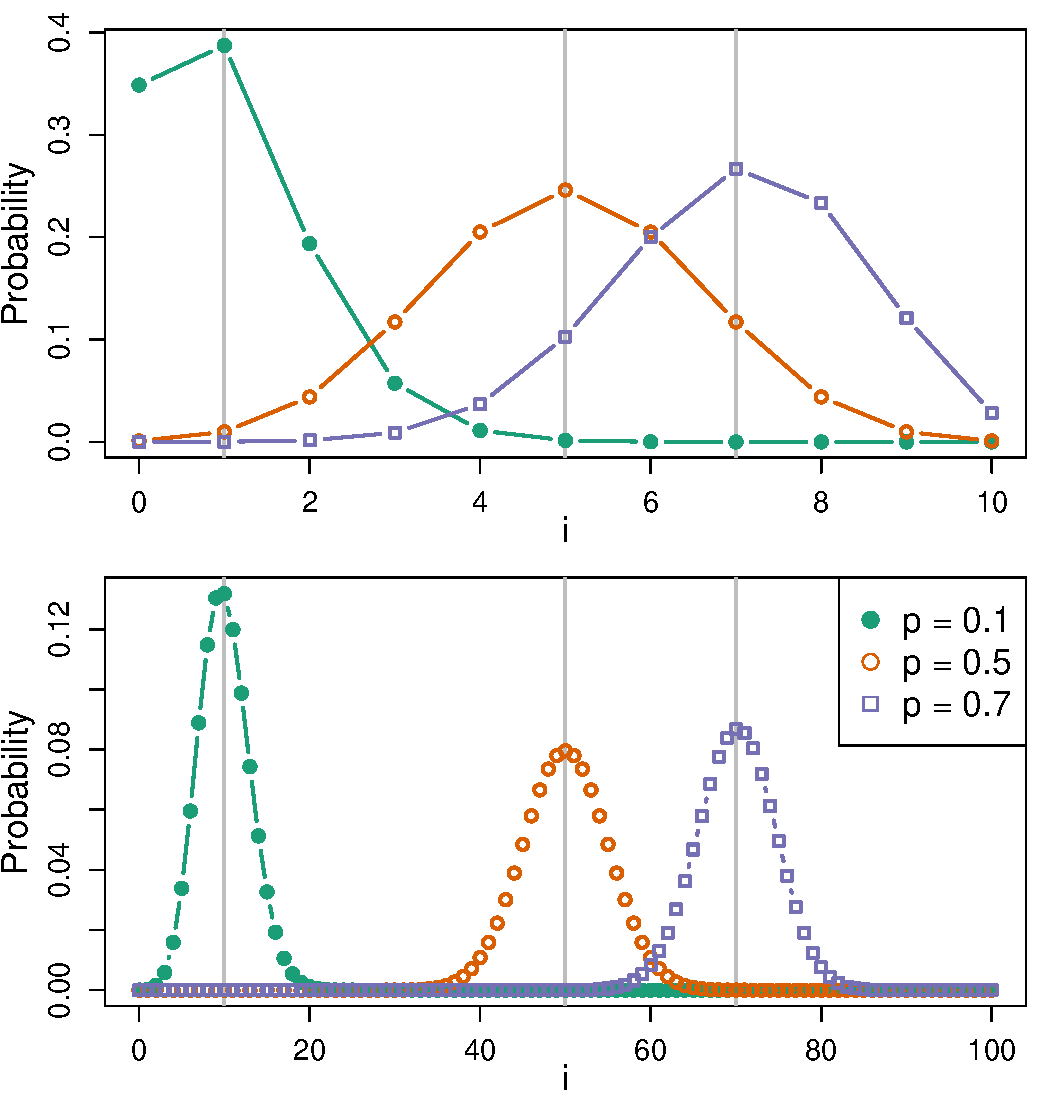
\includegraphics[width=\textwidth]{math_background/dist_pics/Binomial.pdf}\end{center}
 \caption{Binomial distribution for a sample of $n=10$ and $n=100$,
   the vetical lines show the means $np$. \gitcode{https://github.com/cooplab/popgen-notes/blob/master/math_background/Math-background.R}}\label{Fig:binomial}
 \end{marginfigure}

Important discrete random variables include
\begin{description}
\item[Binomial]  random variables count the number $X$ of heads when
  flipping a coin $n$ times whose (biased) probability of being heads is $p$. In which case, 
\begin{equation}
  p_i = \frac{n!}{i!(n-i)!} p^i (1-p)^{n-i} \qquad 0\le i \le n.
\end{equation}
For a binomial random variable, $\E[X]=np$ and
$\sigma^2=np(1-p)$. Examples are shown in Figure \ref{Fig:binomial}, Note how the mass of the
   distribution becomes more centered on the mean for larger sample
   sizes, as the standard deviation increases only as $\sqrt{n}$. 
Another way that we can write that our observation $i$ is drawn from
the binomial distribution is $i \sim
\textrm{Binomial}(p,n)$, where $i \sim$ is read as ``$i$ is
distributed as'' (we will use the notation as short hand for random
variable in the notes).

\item[Geometric] random variables count how many flips $X$ you wait before seeing a heads on a coin with probability $p$ of being heads. In which case, 
\begin{equation}
p_i =p (1-p)^{i-1} \qquad i=1,2,\dots
\end{equation}
    \begin{marginfigure}
 \begin{center}
   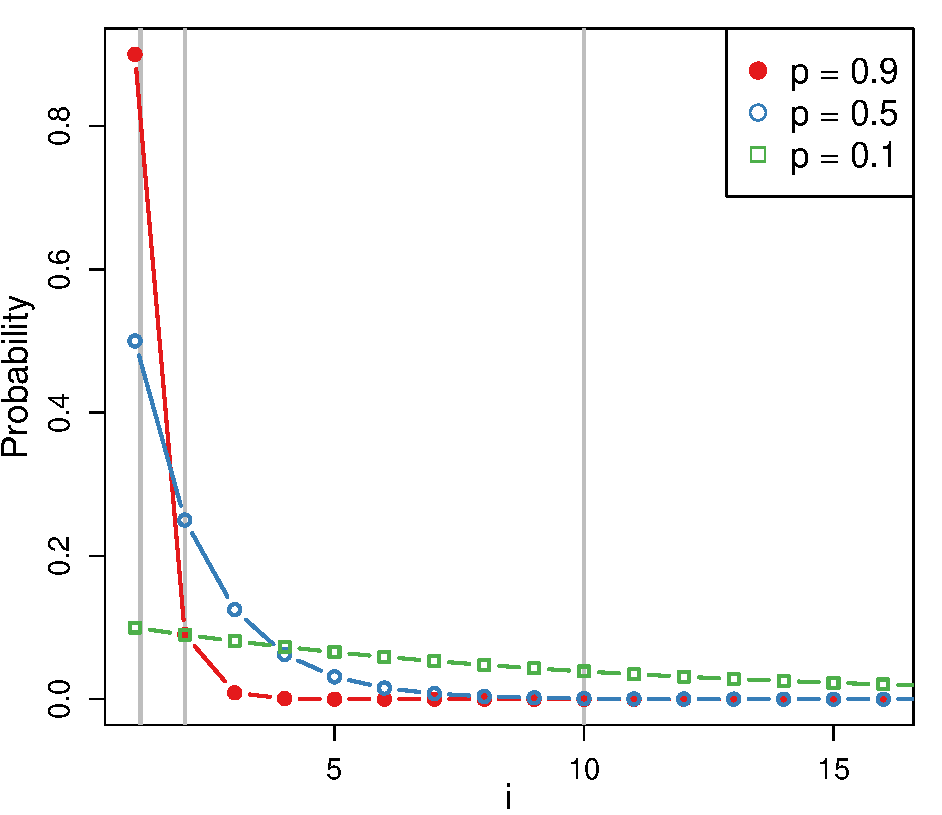
\includegraphics[width=\textwidth]{math_background/dist_pics/Geometric.pdf}\end{center}
 \caption{Geometric distribution for different probabilities of
   success ($p$). The vertical lines show the means $1/p$. \gitcode{https://github.com/cooplab/popgen-notes/blob/master/math_background/Math-background.R}}\label{Fig:geometric}
 \end{marginfigure}
For a geometric random variable $\E[X]=1/p$; if our coin is fair
$p=\nicefrac{1}{2}$ we wait two flips for a head on average while if
the coin-flip is very biased against heads $p \ll 1$ we can be waiting
a very long time. The variance of a
geometric random variable is $\sigma^2 =\nicefrac{1-p}{p^2}$, which
means that the mass of the distribution is much more spread out if we
consider the waiting time for rare events. See Figure
\ref{Fig:geometric} for examples of the distribution. 

\item[Poisson] random variables count the $i$ events that occur in a
  fixed interval of time or space ($t$), when these events occur independently of
  each other and of time. If $\lambda$ events are
  expected to occur in this interval, then
 \begin{equation}
p_i = \lambda^i e^{-\lambda}/i!
\end{equation}
    \begin{marginfigure}
 \begin{center}
   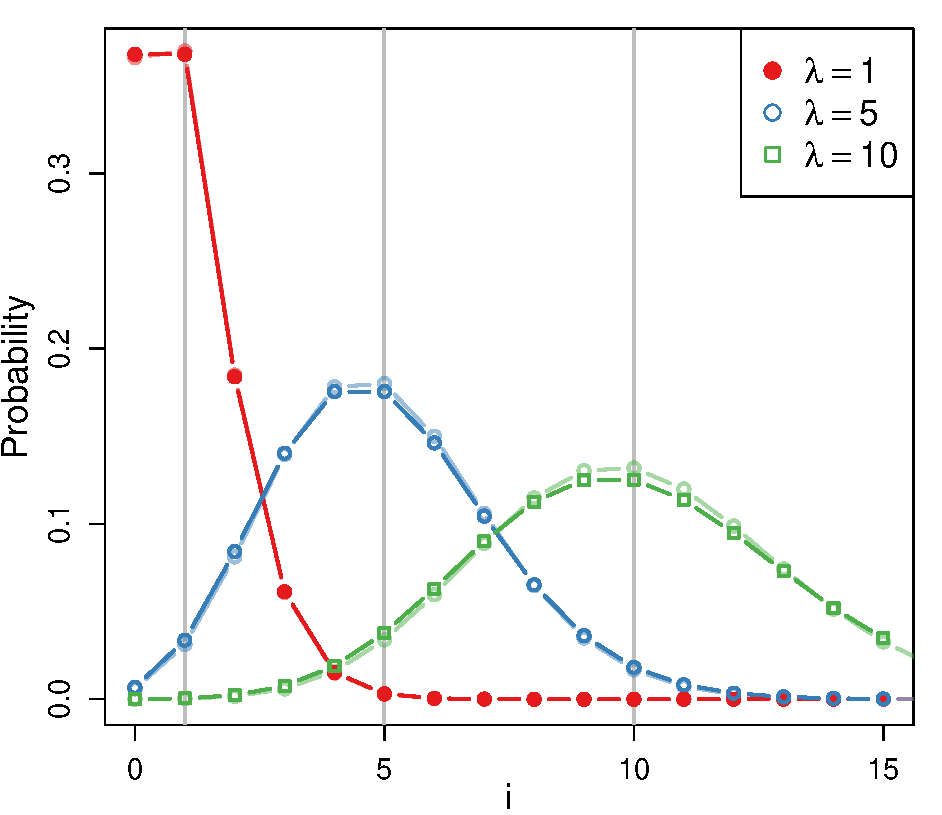
\includegraphics[width=\textwidth]{math_background/dist_pics/Poisson.pdf}\end{center}
 \caption{Poisson distribution with different means ($\lambda$). the
   vetical lines show the means. The lighter coloured lines show a
   binomial with $n=100$ and $p=\nicefrac{\lambda}{n}$ to illustrate
   how well the Poisson approximates the bionomial for rare events
   (it's hard to see them as they are close together!). 
   \gitcode{https://github.com/cooplab/popgen-notes/blob/master/math_background/Math-background.R}}\label{Fig:poisson}
 \end{marginfigure}
 For a random Poisson variable $\E[X]=\lambda$.

 The form of this is less intuitive than that of the (say)
 binomial. However, one way we can derive it is as the limiting case of the
 binomial. Think of setting up a game of chance, where there's a very large number of coin
 flips ($n \rightarrow \infty$), but you've set the chance of heads on a single
 coin flip is very low ($p  \nicefrac{\lambda}{n} \rightarrow 0$,
 where $\lambda$ is a constant).  Under these conditions you'd still
 expect some heads ($np =\lambda$), and the distribution of the number
 of heads is Poisson. See Figure \ref{Fig:poisson} to see how well
 they match. To see this we substitute
 $p=\nicefrac{\lambda}{n}$ into our binomial probability and take
 the limit as $n \to \infty$ 
 \begin{align}
   p_i &= \frac{n!}{i!(n-i)!} p^i (1-p)^{n-i} \nonumber\\
         &= \lim_{n\to\infty} \frac{n(n-1)\ldots
         (n-k-1)}{i!} \left(  \frac{\lambda}{n}\right)^i \left(1-
         \frac{\lambda}{n}\right)^{n-i} \nonumber\\
   & = \lim_{n\to\infty} \frac{n^k}{i!} \frac{\lambda^k}{n^k} \left(
     \frac{\lambda}{n}\right)^n \nonumber\\
 &=  \lim_{n\to\infty} \frac{\lambda^k}{i!} e^{-\lambda}
 \end{align}
 \end{description}
Therefore, the Poisson represents the limit of
the binomial. 
\subsection{Continuous Random Variable Distributions.}
Important continuous random variables include
\begin{description}
\item[Uniform] random variables correspond to ``randomly'' choosing a number in an interval, say $[a,b]$. The pdf for a uniform is 
\begin{equation}
p(x)=\frac{1}{b-a} \mbox{ for }x\in[a,b]\mbox{ and } 0 \mbox{ otherwise.}
\end{equation}
For a uniform random variable $\E[X]=(a+b)/2$.
\item[Exponential] random variables with rate parameter $\lambda>0$ correspond to the waiting time for an event which occurs with probability $\lambda \Delta t$ over a time interval of length $\Delta t$. For these random variables
\begin{equation}
p(x)= \lambda \exp(-\lambda x) \mbox{ for }x\ge 0 \mbox{ and } 0 \mbox{ otherwise.}
\end{equation}
For an exponential random variable $\E[X]=1/\lambda$. The Exponential
distribution is the continuous-time version of the Geometric
distribution. Informally this can be seen by considering the trials in
the geometric distribution as narrow time-intervals and 

\item[Normal] random variables have the ``bell-shaped'' or ``Gaussian'' shaped distribution. They are characterized by two parameters, the mean $\mu$ and the standard deviation $\sigma$, and
\begin{equation}
p(x)=\frac{1}{\sigma\sqrt{2\pi}}\exp(-(x-\mu)^2/(2\sigma^2)).
\end{equation}
For a normal random variable $\E[X]=\mu$. 
\end{description}

\subsection*{Multiple random variables}

\paragraph{Covariance and Independence} To fully specify multiple random variables, say $X$ and $Y$, one needs to know their joint distribution. For example, if $X$ and $Y$ are discrete random variables taking on the values $x_1,x_2,x_3,\dots$, then the joint distribution is given by 
\begin{equation}
p_{i,j}=\P[X=x_i,Y=x_j] \mbox{ `` the probability that $X$ equals $x_1$ and $Y$ equals $x_2$''}
\end{equation}
for all $i$ and $j$, see also our discussion around eqn. \eqref{eqn:basic_indie}.

Alternatively, if $X$ and $Y$ are continuous random variables, then the joint distribution is a function of the form $p(x,y)$ which satisfies 
\begin{equation}
\P[a\le X\le b, c\le Y\le d]= \int_a^b \int_c^d p(x,y)\,dxdy. 
\end{equation}
where $X$ and $Y$ are said to be independent if we can write the
joint density as a product of the probability density functions 
\begin{equation}
p(x,y) = p(x) p(y).
\end{equation}

Given any function $f(x,y)$ of $x$ and $y$, one can define the expectation $\E[f(X,Y)]$ by integrating with respect to the distribution. Namely, 
\begin{equation}
\E[f(X,Y)]=\int \int f(x,y)p(x,y)\,dxdy \mbox{ for continuous case and } \sum_i \sum_j f(x_i,x_j) p_{i,j} \mbox{ in discrete case}
\end{equation}

The \emph{covariance} of  $X$ and $Y$ is given by 
\begin{equation}
\E[(X-\mu_X)(Y-\mu_Y)]=\E[XY]-\mu_X\mu_Y. 
\end{equation}
$X$ and $Y$ are said to \emph{uncorrelated} if their covariance equals
zero.If $X$ and $Y$ are independent, then they are guaranteed to be
uncorrelated, but it is possible to construct $X$ and $Y$ to be
uncorrelated but not independent. 


\paragraph{Sample Covariance and Correlation} 
We can calculate the \emph{sample covariance} for $X$ and $Y$ of a set of observations
of $X_1, \cdots, X_L$ and $Y_1, \cdots, Y_L$, where these observations
are paired $(X_i,~Y_i)$ as
\begin{align}
 \widehat{\sigma_{XY}^2}  &= \frac{1}{L-1} \sum_{i=1}^L (X_i -
                            \bar{X}) (Y_i - \bar{Y})  %\nonumber\\
  %&= \left( \frac{1}{L-1} \sum_{i=1}^L X_iY_i \right) - \bar{X} \bar{Y}
\end{align}
this captures the extent to which two sets of numbers covary. For
example, the running speeds of kids in a race at age 8 and 9 positively
covary. Example datasets are shown in Figure \ref{Fig:Covar_egs}. 

    \begin{figure}
 \begin{center}
   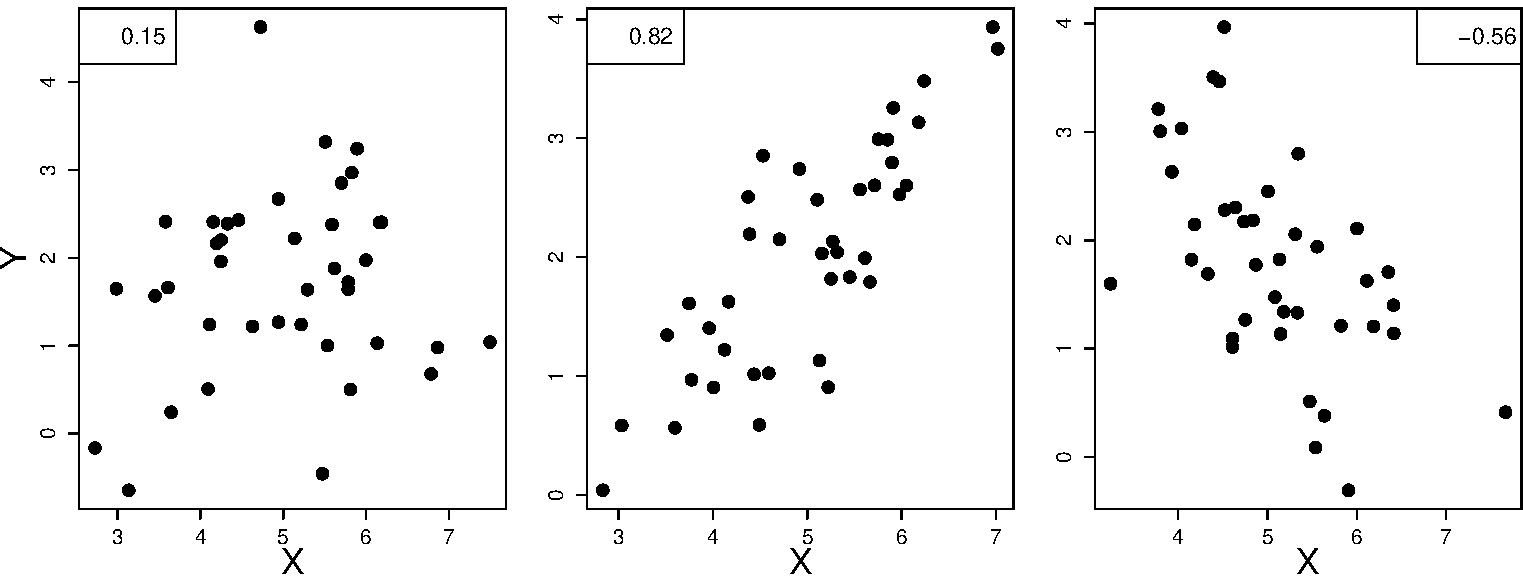
\includegraphics[width=\textwidth]{math_background/dist_pics/Covar.pdf}\end{center}
 \caption{Examples of datasets where pairs of variables show varying
   degrees of covariance, the sample correlation ($ \widehat{\rho_{XY}}$) is shown in the top corner.
   \gitcode{https://github.com/cooplab/popgen-notes/blob/master/math_background/Math-background.R}}\label{Fig:Covar_egs}
 \end{figure}
To move covariances to a more understandable scale we can divide
through by the product of the standard deviations
\begin{equation}
\rho_{XY} = \frac{{\sigma_{XY}}}{\sigma_{X} \sigma_{X}}
\end{equation}
this is the \emph{correlation} of our variables $X$ and $Y$, if we
calculate it for our sample it is our \emph{sample correlation}. A correlation can range between $1$,
perfectly correlated, to $-1$ perfectly negatively correlated. If
$\rho_{XY} =0$ the variables are said to be uncorrelated.

\paragraph{Fitting a linear regression using least squares.}
We often want to approximate the relationship between our two variables
$X$ and $Y$ by the best fitting linear relationship predicting $Y$
value from their observed $X$
value. For example, think of a linear prediction of a child's weight from their height. 
See Figure \ref{Fig:Regression_eg} for an example plot. To do this we can think of approximating the $Y_i$ that
accompanies the $X_i$ value for the $i^{th}$ pair of data points by
\begin{equation}
Y_i \approx a+ b X_i 
\end{equation}
where $a$ and $b$ are the intercept and slope of a line.

 \begin{marginfigure}
 \begin{center}
   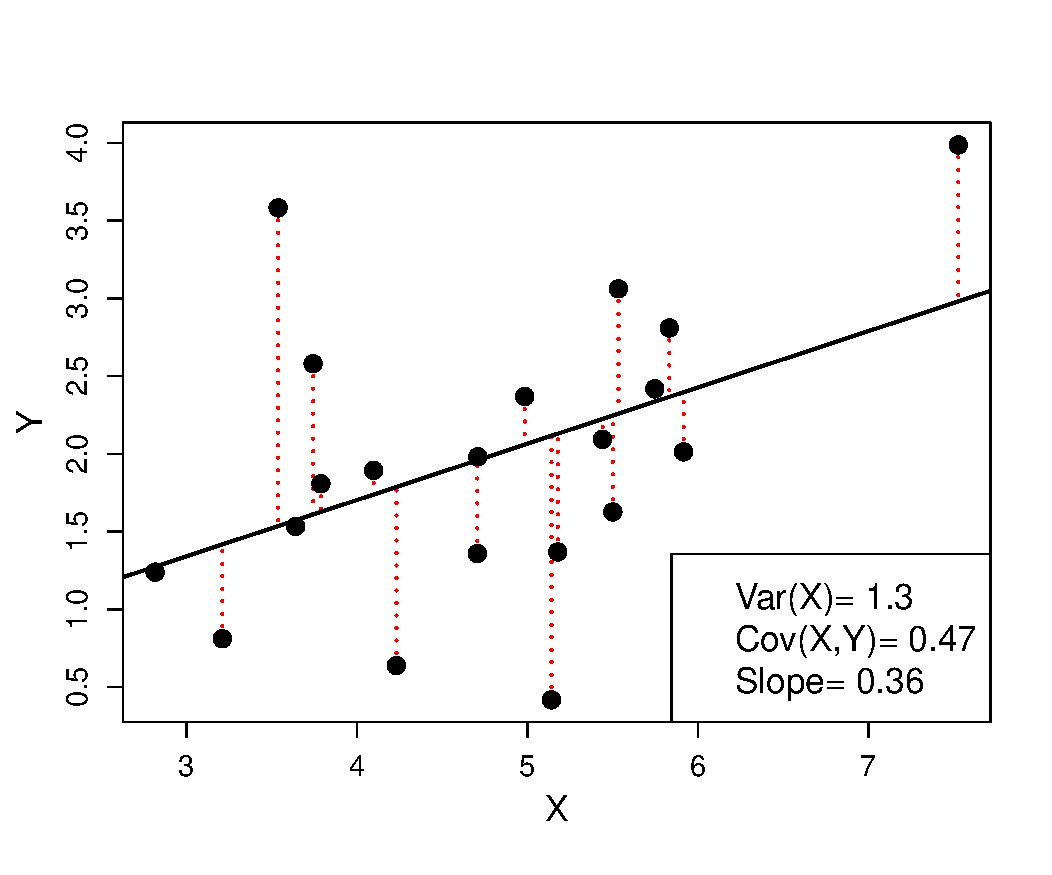
\includegraphics[width=\textwidth]{math_background/dist_pics/Linear_regression.pdf}\end{center}
 \caption{An example of a linear regression with best fitting
   least-squares line. The sample variance and covariance are given,
   so that you can see for yourself that the best fitting slope is
   just the ratio of these two. 
   \gitcode{https://github.com/cooplab/popgen-notes/blob/master/math_background/Math-background.R}}\label{Fig:Regression_eg}
 \end{marginfigure}

What
is the best fitting line? Well one common definition of the optimal fit is
the choice of $a$ and $b$ that minimize the squared error
between the observed ($Y$) and their predicted values, i.e.
\begin{equation}
\sum_{i=1}^L  (Y_i  - a -  b X_i )^2
\end{equation}
here $(Y_i  - a -  b X_i)^2$ is the squared residual error, the square
of the length of the dotted lines in Figure
\ref{Fig:Regression_eg}. The best fitting slope, i.e. that with least
squared error, is
\begin{equation}
b = \nicefrac{ \widehat{\sigma_{XY}^2}}{ \widehat{\sigma_{X}^2}} \label{eqn:slope_linear_reg}
\end{equation}
i.e. the sample covariance of $X$ and $Y$ divided by the sample
variance of $X$. Thus the slope will be of the same sign as the
covariance, and will be larger in magnitude when the covariance of $X$
and $Y$ is a large proportion of the variance of $X$.

This least squares fit is the solution to the linear regression
\graham{Doc points out  The conditions here are the ones for it to be BLUE, which is hard to convey easily. (And tbh kind of misleading, since the form of "linearity" inherent in the "L" is actually super restrictive) Consistency is maybe easier to convey---you could say something about it being consistent under x,y circumstances.}
\begin{equation}
Y_i \sim a+ b X_i + \epsilon_i
\end{equation}
where the errors ($\epsilon_i$) are uncorrelated across data points
with an expectation of zero and constant but unknown variance. These
assumptions would hold for example if $\epsilon_i \sim \textrm{Normal}(0,\sigma)$.


We often want to include additional terms in our regression, or have
more complicated error structures, but these
extensions can usually be understood as simple extensions of this
machinery. For example, least-squares can also be used to fit a non-linear
function of $X$, $f(X,~\Omega)$, 
where we minimize 
\begin{equation}
\sum_{i=1}^L  (Y_i  -f(X_i; ~\Omega ))^2
\end{equation}
over our choices of parameters $\Omega$. Often there is no analytical
solution, i.e. no equivalent of eqn. \ref{eqn:slope_linear_reg}, and
the answer must be found computationally (with easy tools available in
R and other programming languages). Throughout the book we use
non-linear least squares to fit various models to data. 

%It can be show, for example in the discrete case, this is equivalent to 
%\begin{equation}
%\P[X=x_i\mbox{ and } Y=x_j]=\P[X=x_i]\P[Y=x_j]
%\end{equation}
%for any $i,j$.

\subsection*{Other useful results.}
\paragraph{Law of Large Numbers} If $X_1,X_2,\dots$ are a sequence of independent random variables (i.e. ``the outcomes of a sequence of independent experiments) with common expectation $\mu= \E[X_i]$, then 
\begin{equation}
\frac{X_1+\dots +X_n}{n} \to \mu \mbox{ as }n\to \infty \mbox{ with
  probability one.}
\end{equation}
Hence, LLN implies that if you repeat a bunch of experiments and take the average outcome from the experiments, the value you get is likely to be close the expected outcome of the experiment. 

Of course, in the real world, we can only perform a finite number of experiments in which case it is useful to have a sense of how much variation there will be in the average outcome. The central theorem is the key tool for understanding this variation. 

\paragraph{Central Limit Theorem} If $X_1,X_2,\dots$ are a sequence of independent random variables (i.e. ``the outcomes of a sequence of independent experiments) with common expectation $\mu= \E[X_i]$ and variance $\sigma^2$, then 
\begin{equation}
\frac{X_1+\dots +X_n-\mu \,n }{\sqrt{n}\sigma} \to \mbox{ normal distribution with mean $0$ and variance $1$ as $n\to \infty$ }
\end{equation}
Hence, for $n$ large enough 
$
X_1+\dots+X_n 
$
is approximately normally distributed with mean $\mu\,n$ and variance $\sigma^2 n$. 
